\section{Resilience Quantification}
\label{sec:resilience}

Loosely, resilience refers to the capacity for a system to retain its overall qualitative structure in the face of disturbances. Its precise definition differs between authors and disciplines; an abundance of approaches to quantifying resilience have been proposed. 
%
In this section, I define asymptotic resilience and intensity of attraction. 
%
For a review of some other mathematical definitions of resilience that I do not cover, see \cite{meyerMathematicalReviewResilience2016}.


\subsection{Preliminaries}
Let $U \subset \mathbb{R}^n$ be an open set, and assume that $f : U \to \mathbb{R}^n$ is a locally Lipschitz continuous function which is continuously differentiable. Consider a system of ordinary differential equations (ODEs) 

\begin{equation}
	\label{eqn:ode}
	x' = f(x)
\end{equation}

The Lipschitz condition guarantees well-defined solutions, but only for sufficiently short intervals of time; hence we call the solutions \textbf{local}. We will use flow notation to collect all solution trajectories into one convenient object, called the \textbf{local flow} $\varphi: D \subset \mathbb{R} \times U \to U$, which is defined such that $\varphi(t,x_0) = x(t)$ is a solution to the initial value problem \begin{center}
	$x'(t) = f(x(t))$, \hspace{0.25in} $x(0) = x_0$. 
\end{center}

Depending on context, $f$ may be globally Lipschitz continuous, in which case trajectories are defined for as long as they remain within the domain $U$. If no trajectories leave $U$, then $\varphi$ is a \textbf{global flow}, meaning it is defined for all time. In this paper we will simply assume for convenience that the flow is defined on any time domain of interest. 

Additionally, we will be taking the following notational conveniences. For a flow $\varphi$, we will denote the time-$t$ map as $\varphi_t: U \to U$. We will naturally extend this notation to allow set-valued inputs $S\subset U$: $$\varphi_t(S) = \{x\in U ~| ~\varphi_t(x_0) = x \text{ for some } x_0 \in S\}.$$

Intuitively, the map $\varphi_t$ outputs the location of any input point after it flows for $t$ units of time. If the input is a set, then the output is also a set, consisting of all the locations reached at time $t$.

Two central objects of study in this paper are attractors and their associated basins of attraction. Attractors characterize the system's behavior as $t \to \infty$, by pulling trajectories toward them -- at least, those trajectories which begin within their basin of attraction. Tipping behavior often comes down to either an abrupt shift in the nature of an attractor or an abrupt switch from one attractor to an alternative attractor. When we talk about resilience in this paper, we are referring to the resilience \textit{of an attractor}. 

In order to define attractors and basins, we must first formalize some aspects of long-term behavior.

\begin{definition}
	Consider a subset $S \subset U$. 
	%$S$ is \textbf{forward invariant} under the flow $\varphi$ if it contains all its forward images in time: $\varphi_t(S) \subset S$ for all $t \in \mathbb{R}^+$. Similarly, $S$ is \textbf{backward invariant} if $\varphi_t(S) \subset S$ for all $t \in \mathbb{R}^-$. $S$ is \textbf{invariant} if it is both forward and backward invariant. 
	$S$ is \textbf{invariant} under the flow $\varphi$ if it contains all its own images in time: $\varphi_t(S) \subset S$ for all $t \in \mathbb{R}$.
	\qed
\end{definition}

Intuitively, an invariant set is one which always stays put. %while forward and backward invariant sets stay put in forward and backward time, respectively. 
The next definition describes where an arbitrary set ends up, or at least limits toward, in the long tun. 

\begin{definition}
	The \textbf{omega limit set} of $S \subset U$ is $$\omega(S)
	= \bigcap \limits_{T > 0} \overline{ \bigcup\limits_{t > T} \varphi_t(S) }.$$ \qed
\end{definition}

%The omega limit set describes where trajectories that begin in $S$ eventually limit toward in forward time. Now we are ready to define an attractor. Additionally, an attractor has an associated domain, or basin of attraction, which is the subspace attracted to it. 

Now we have the vocabulary to formally define attractors and basins.

\begin{definition}
	An \textbf{attractor} $A \subset U$ is a non-empty, compact, invariant set which is the omega limit set $\omega(N)$ of some neighborhood $N$ of itself. Its \textbf{basin of attraction}, also called its \textbf{domain}, is $$basin(A) = \{x \in U ~|~ \omega(x) \subset A, \omega(x) \neq \emptyset\}.$$ \qed
\end{definition}

As mentioned, attractors are the fixed structures in a system which are approached by solution trajectories in the long run. Each attractor has a certain dominion of rule -- those trajectories beginning within its basin are the ones that end up drawn toward it. While attractors may have interesting structures -- periodic or chaotic, for instance -- we will begin with the simplest type of attractor: an \textbf{attracting rest point}. These attracting rest points, also called \textbf{stable rest points}, capture the intuitive idea of a "steady state." 

The next definition says that a rest point is any unmoving point, while the subsequent proposition, which is standard theory, gives conditions under which a rest point is an attracting one. 

\begin{definition}
	$x_\ast$ is a \textbf{rest point} or \textbf{equilibrium} of the ODE (\ref{eqn:ode}) if $f(x_\ast) = 0$.
\end{definition}

%\begin{definition}
	%A rest point $x_\ast$ is a \textbf{asymptotically stable} if
%\end{definition}

\begin{proposition}
	If all eigenvalues of linearization at the rest point $x_{\ast}$ have negative real part, that is, $$Re(\lambda) < 0 \text{ for all } \lambda \in spec(\textbf{D}f(x_\ast)),$$ 
then $x_{\ast}$ is an attractor. %Note: we also call such an $x_\ast$ a \textbf{stable rest point}. \todo{what is the best terminology here?} 
\qed
\end{proposition}

Finally, we give useful terminology to classes of rest points which do not fall into the above category. 

\begin{definition}
	If all eigenvalues of linearization at the rest point $x_{\ast}$ have non-zero real part, then $x_{\ast}$ is called \textbf{hyperbolic}. Otherwise, at least one eigenvalue has zero real part, and we call $x_{\ast}$ \textbf{non-hyperbolic}.
	\qed
\end{definition}

\begin{definition}
	If $x_{\ast}$ is hyperbolic, and at least one eigenvalue of linearization at the rest point $x_{\ast}$ has positive real part, then $x_{\ast}$ is called \textbf{unstable}. 
	\qed
\end{definition}

Hyperbolic rest points can be thought of as ``nice" rest points, ones near which the dynamics are predictable in some sense. Unstable rest points match the intuitive notion of unstable states -- around them, nearly all trajectories are repelled away. At non-hyperbolic points the behavior is unpredictable -- the point may be stable, unstable, or neither. 

This concludes our set up of the preliminary framework, and we continue next to the definitions of asymptotic resilience and intensity of attraction.

\subsection{Asymptotic Resilience}
\label{sec:asymp_res}

Throughout this subsection, we will assume that $x_\ast$ is an attracting rest point of a continuously differentiable ODE. Probably the most commonly used mathematical definition of resilience,  originating in theoretical ecology \cite{pimmComplexityStabilityEcosystems1984, mayStabilityComplexityModel1974, hollingResilienceStabilityEcological1973, pimm1991balance}, represents long-term return rates to $x_{\ast}$, and is measured by (the real part of) the dominant eigenvalue at linearization. 

\begin{definition}
	\label{def:asymp}
	 Let $\textbf{A} = Df(x_\ast)$ denote the Jacobian, and recall that all eigenvalues of $\mathbf{A}$ have negative real part. Let $\lambda_1(\textbf{A})$ be the eigenvalue with largest (closest to 0) real part. 	The \textbf{asymptotic resilience} of the system at the stable rest point is equal to the negative of that real part, $$-Re(\lambda_1(\textbf{A})).$$

Note: we will refer to $\lambda_1$ as the \textbf{dominant eigenvalue} or the \textbf{slow eigenvalue} of $\mathbf{A}$. 
	 \qed 
\end{definition}

For the linearized system $x'= \textbf{A}x$, asymptotic resilience estimates the rate at which trajectories approach the equilibrium. The following theorem is standard theory for linear ODEs. %See for example (Chicone p. 175) \todo{do citation}


\begin{theorem}
	For an $n \times n$ matrix $\mathbf{A}$, if $Re(\lambda) < L < 0$ for all eigenvalues $\lambda$ of $\mathbf{A}$, then there is some constant $C>0$ such that for all $x \in \mathbb{R}^n$ and $t \geq 0$,
	%
	$$|e^{t\mathbf{A}}x| \leq Ce^{L t}|x|.$$ 
	%
	And in the long term $C$ can be taken to equal $1$. That is, there is some $T \geq 0$ such that
	%
	$$|e^{t\mathbf{A}}x| \leq e^{L t}|x| ~ ~\text{ for all } t \geq T.$$
	
	%Further, in the limit, and for all $x$ except on a set of measure 0, the inequality can be replaced with equality and $L$ can be replaced with asymptotic resilience.
	%
	%$$\lim\limits_{t \to \infty} |e^{tA}x| = e^{Re(\lambda_1) t}|x| ~ ~\text{ for almost all } x.$$ \todo{make sure this last part is true and include a proof in the appendix}
	
	 \qed
\end{theorem}


%TO DO: Is there a converse to the inequality? how to say that this is a good bound? i.e. for almost all trajectories, and in the limit as $t\to \infty$, they do eventually decay at that rate, rather than much faster than it. I feel like this is true, but I can't find a statement of it in a book. \todo{to do}

%\begin{theorem}
%	For an $n \times n$ matrix $\mathbf{A}$, if $Re(\lambda) < L < 0$ for all eigenvalues $\lambda$ of $\mathbf{A}$, then there is some constant $T>0$ such that for all $x \in \mathbb{R}^n$ and $t \geq T$,
%	
%	$$|e^{tA}x| \leq e^{L t}|x|.$$  \qed
%\end{theorem}

Note the operator $e^{t\mathbf{A}}$ in the left hand side is exactly the flow $\varphi_t$ for the linear system $x' = \mathbf{A}x$. So this theorem says that, in the long term, trajectories must decay to the origin at an exponential rate governed by the asymptotic resilience. 

%A related theorem serves as a converse of sorts, and says that the exponential bound is a good bound, so that trajectories typically do not decay significantly faster. A proof is contained in the appendix.  \todo{Is this correct? Need to work through a proof carefully. I can't find this in a book.}
%
%\begin{theorem} For almost all initial conditions $x\in U$, and in the limit as $t \to \infty$,
%	$$ |e^{tA}x| = e^{ Re(\lambda_1)t}|x|.$$ \qed
%\end{theorem}

%\begin{theorem}
%	For almost all initial conditions $x_0 \in U$, 
%	$$\lim\limits_{t \to \infty} |\varphi_t(x_0)|' = Re(\lambda_1)|\varphi_t(x_0)|,$$
%	where $' = \dfrac{d}{dt}$, and $\lambda_1$ is the dominant eigenvalue of $\mathbf{A}$.
%\end{theorem}

%\todo{write proof.}

For nonlinear systems, similar results for decay rate are justified by the Stable Manifold Theorem, a fundamental result which says that, at sufficiently nice rest points, the linear approximation is a good approximation. 
%
%The theorem states that there is a local  Moreover, the flow restricted to the stable and the unstable manifolds has exponential (hyperbolic) estimates similar to the inequalities in display (4.1)
%
%
A special case of the Stable Manifold Theorem is stated here, while a full version can be found in any standard text. %is relegated to the appendix. 

\begin{theorem}(Stable Manifold Theorem, for attracting rest points)
	Consider a non-linear system 
	%
	$$x' = \mathbf{A}(x) + h(x),$$ 
	%
	where $\mathbf{A}, h: \mathbb{R}^n \to \mathbb{R}^n$ with $\mathbf{A}$ linear.  Let $\phi_t$ be the local flow.
	%
	Assume there is an attracting rest point at the origin. 
	%
	Let $\lambda_1$ be the dominant eigenvalue of $\mathbf{A}$. Then there exists a neighborhood $N \ni 0$ which is a \textbf{local stable manifold} of the origin. 
	%
	That is, for all $x \in N$, $\lim\limits_{t \to \infty} \phi_t(x)= 0$.
	
	Furthermore, for any $Re(\lambda_1) < L < 0$, there exists $C >0$ such that for all $x \in N$, $t \geq 0$,
	%
	$$|\phi_t(x)| \leq Ce^{Lt}|x|,$$
	%
 	and for some $T \geq 0$, $C$ can be taken to equal $1$
	%
	$$|\phi_t(x)| \leq e^{L t}|x| ~ ~\text{ for } t \geq T.$$
	%Finally, in the limit, and for all $x\in N$ except on a set of measure 0, the inequality can be replaced with equality and $L$ can be replaced with asymptotic resilience.
	%
	%$$\lim\limits_{t \to \infty} \phi_t(x)| = e^{Re(\lambda_1) t}|x| ~ ~\text{ for almost all } x.$$ \todo{make sure this last part is true and include a proof in the appendix}
	\qed
\end{theorem}

%TO DO: does that last statement about long term $C=1$ hold? Can't find this in a book but I feel like it should be true. And also, what about a converse to the inequality? Does anything like that exist for the stable manifold theorem, if it does for linear systems? \todo{to do}

The theorem implies that any trajectory beginning sufficiently close to equilibrium decays toward equilibrium at an exponential rate, where that rate is determined in the long term by asymptotic resilience. Any point which is very close to, but not quite at, the equilibrium represents a state slightly perturbed away from steady state. Hence, the rate of decay can be thought of as the recovery rate from a small perturbation. 

%Hence, asymptotic resilience bounds the rate of return to equilibrium after a small perturbation to the system. Because local bifurcation is characterized by $Re(\lambda_1)$ passing through zero, the system recovers slower when nearer to bifurcation. This is the core idea of critical slowing down, which will be explained further in Section \ref{sec:csd}.

\begin{remark}
	Note that trajectories need not decay monotonically in distance to the rest point, not even for linear systems. For instance, a trajectory can initially amplify in magnitude -- a phenomenon termed \textbf{reactivity} by Neubert and Caswell in \cite{neubertAlternativesResilienceMeasuring1997} (Figure \ref{fig:reactivity}). However, with some large enough choice of $T$, the Stable Manifold Theorem still implies that short term growth negligibly affects long term decay. 
\end{remark}	

\begin{figure}[ht]
	\centering
	\captionsetup{width=0.8\linewidth}
	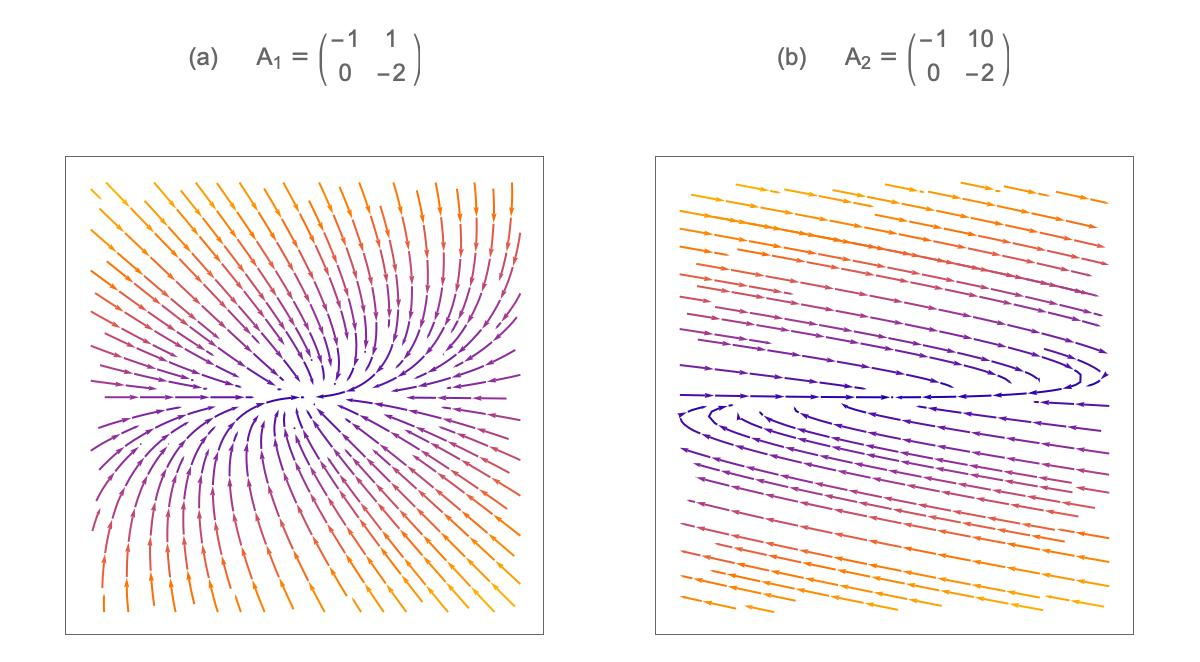
\includegraphics[width=0.8\textwidth]{figs/positive_reactivity_real_example}
	\caption{Phase portraits of two linear systems $x' = \textbf{A}x$. (a) All trajectories decay monotonically in magnitude. (b) There are trajectories beginning arbitrarily close to the origin which initially increase in magnitude. Notice that both matrices have the same eigenvalues $\lambda = -1, -2$; hence asymptotic resilience cannot tell whether an equilibrium is reactive. Example reproduced from \cite{neubertAlternativesResilienceMeasuring1997}.}
	
	\label{fig:reactivity}
\end{figure} 

%\subsection{Reactivity}
Asymptotic resilience governs the long-term rate of recovery. However, in the short term, perturbations can initially be amplified before eventually decaying to the stable equilibrium (Figure \ref{fig:reactivity}). Motivated by this transient behavior, an alternative measure of system response to perturbations was introduced by Neubert and Caswell in \cite{neubertAlternativesResilienceMeasuring1997a}.

\begin{figure}[ht]
	\centering
	\captionsetup{width=0.8\linewidth}
	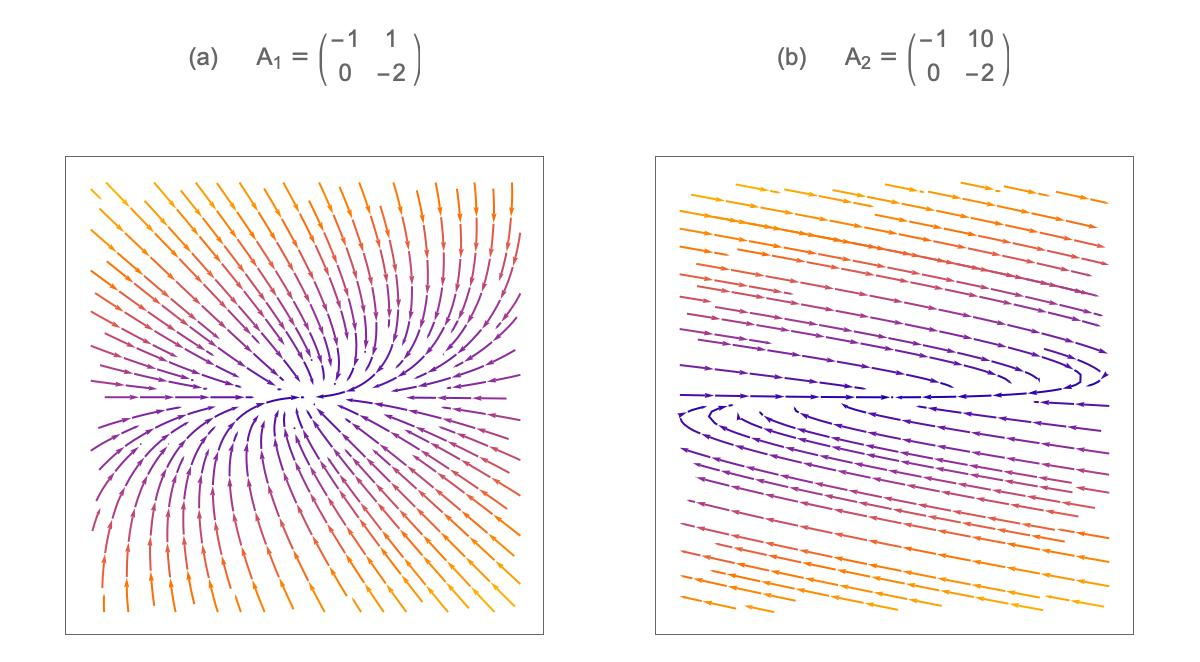
\includegraphics[width=0.8\textwidth]{figs/positive_reactivity_real_example}
	\caption{Phase portraits of two linear systems $x' = \textbf{A}x$ with the same eigenvalues  $\lambda = -1, -2$. (a) All trajectories decay monotonically in magnitude. (b) Trajectories may transiently increase in magnitude before decreasing. Example reproduced from \cite{neubertAlternativesResilienceMeasuring1997a}.}
	
	\label{fig:reactivity}
\end{figure} 

\begin{definition}
	Suppose that $x_\ast$ is a stable rest point of the ODE (\ref{eqn:ode}). Let $\textbf{A} = Df(x_\ast)$ be the Jacobian, and let $\textbf{H} = \frac{\textbf{A}+\textbf{A}^T}{2}$ be its symmetric part. Since $\textbf{H}$ is a real symmetric matrix, it has real eigenvalues. Let $\lambda_1(\textbf{H})$ be the maximum eigenvalue.
	
	 \begin{center}
	 	The \textbf{reactivity} of the system at the stable rest point is $\lambda_1(\mathbf{H})$.\\ If this number is positive, the system is called \textbf{reactive}.
	 \end{center}
	
	\qed
\end{definition}

Reactivity measures the maximum possible relative rate of initial amplification. The following proposition, which relies on elementary linear algebra, shows this result for linear systems. 

\begin{proposition}[Neubert and Caswell]
	For the linear system $x' = \mathbf{A}x$, $\lambda_1(\mathbf{H}) = \max\limits_{x\in \mathbb{R}^n \setminus \{0\}} \dfrac{||x||'}{||x||}$.
\end{proposition}

\begin{proof}	
	\begin{align*}
		\dfrac{||x||'}{||x||} 	&= \dfrac{1}{||x||} \dfrac{d}{dt}\big(x^Tx\big)^{1/2} \\
										&= \dfrac{1}{2||x||^2} (x^T x' + (x')^T x) \\
										&=  \dfrac{1}{2||x||^2} (x^T \mathbf{A}x + x^T\textbf{A}^Tx) \\
										&= \dfrac{ x^T\mathbf{H}x}{||x||^2}
	\end{align*}

	This expression is a scale invariant function of $x$, so to maximize it, we only need to consider unit vectors. $$\max\limits_{||x||=1} x^T \mathbf{H} x$$
	%
	
	$\mathbf{H}$ is real symmetric, hence diagonalizable with an orthogonal change of basis. Let $\{\lambda_1, \lambda_2, \ldots \lambda_n\} = spec(\mathbf{H})$, in order from largest to smallest.
	\begin{align*}
		x^T\mathbf{H}x &= x^T(\mathbf{BDB}^T)x\\
		&= (x^T\mathbf{B})\mathbf{D}(\mathbf{B}^Tx)\\
		&= y^T \mathbf{D}y, ~\text{  where } y = \mathbf{B}^Tx \text{ is also unit.}\\
		&= \lambda_1 y_1^2 + \lambda_2 y_2^2 + \ldots +\lambda_n y_n^2.
	\end{align*}
The maximum of this expression over all $||y||=1$ is clearly $\lambda_1$, when $y= (y_1, \ldots , y_n) =(1, 0, \ldots, 0)$.

	
	%Since $\mathbf{H}$ is a symmetric matrix, it defines a quadratic form $Q(x) = x^T \mathbf{H} x$. The maximum value of a quadratic form restricted to the unit sphere is the largest eigenvalue of its matrix representation. \todo{cite}
	
\end{proof}

%If a linear system has positive reactivity, then there are arbitrarily small perturbations that will initially amplify, before eventually decaying to the sink. 



to do: relation between nonlinear and linearized systems

%connection to SVD?

% connection to Turing instability?





\subsection{Intensity of Attraction}

Asymptotic resilience notably relies on linearizing at a point attractor. In contrast, intensity of attraction, introduced by Katherine Meyer in her PhD thesis \cite{meyerMetricPropertiesAttractors2019}, measures resilience not only for rest points but also for any other type of attractor. Even more importantly, it captures metric information across the entire basin of attraction rather than simplifying to a topologically equivalent approximation within a limited neighborhood. We now review the necessary background in order to define intensity of attraction. 

First of all, the idea of perturbation will now be represented by what is known as a \textbf{control function} added to an underlying vector field. This construction allows for perturbations which are not necessarily small and isolated, but possibly large and continuous, reflecting important types of perturbation that commonly occur in ecological and other applied settings, such as environmental forces or human-driven pressure (intentional or unintentional) on an ecosystem. We assume that the control function $$g: I \subset \mathbb{R} \to \mathbb{R}^n$$ is taken from the space of essentially bounded (i.e. bounded except on a set of measure 0) measurable functions $L^\infty (I,\mathbb{R}^n)$, where the norm is 
$$||g||_\infty = \inf\{C \geq 0  :  ||g(x)|| \leq C  \text{ for almost every } x \in I \}.$$ 
We also assume $g$ is locally integrable (i.e. integrable on every compact subset of its domain $I$). These mild assumptions will ensure that $g$ is nice enough for our perturbed system to remain well-defined. Next, we formalize how the perturbation is added to an underlying system. 

\begin{definition}
	A \textbf{bounded control system} \todo{is this ok terminology?} is a non-autonomous ODE 
	\begin{equation}
		\label{eqn:control_ode}x' = f(x) + g(t)
	\end{equation}
	where $f: U \subset \mathbb{R}^n \to \mathbb{R}^n$ is locally Lipschitz, $g \in L^\infty (I,\mathbb{R}^n)$ is locally integrable, and its norm $||g||_\infty$ is finite. \todo{how can $g$ have infinite norm and be locally integrable? do i need this as a separate condition?} \qed
\end{definition}

Here, the idea is that there is an underlying ODE $x'=f(x)$, but it is altered by adding the perturbation $g(t)$ to the vector field $f(x)$ on the right hand side. At every point in time, $g(t)$ will adjust the path of solutions somewhat away from their original trajectory. 

It remains to be justified whether such an addition leaves a well-defined system. Because the right hand side $f(x) + g(t)$ may be a discontinuous function, solutions $x(t)$ of the ODE must be considered in an extended sense, which is that $x'(t) = f(x) + g(t) \text{ almost everywhere.}$ Fortunately, the conditions on $g$ are enough to guarantee local existence and uniqueness of solutions in such an extended sense. Briefly: (1) the hypotheses of Caratheodory's theorem are satisfied, establishing existence, and (2) boundedness of $g$ guarantees Lipschitz continuity (local if $f$ is locally Lipschitz, global if $f$ is globally Lipschitz), thereby implying uniqueness. 

So we have well-defined solutions, and can therefore extend the standard local flow notation to the bounded control setting. Fixing an underlying vector field $f$, we will denote as follows the flow obtained by applying a choice of perturbation $g$.

\begin{definition} 
	$\varphi_g(t, x_0): D \subset \mathbb{R} \times U \to U$ is the local flow defined by $$\varphi_g(t, x_0) = x(t)$$ where $x(t)$ solves in the extended sense the ODE (\ref{eqn:control_ode}), with initial condition $x(0) = x_0$. \qed
\end{definition}

Intensity of attraction considers not just one single control function, but entire families of control functions -- specifically, those where every function is bounded by some maximum magnitude $r$. Supposing that vector field perturbations are limited by some ceiling $r$ on magnitude, each family can be thought of as a collection of all possible perturbations. The next definition gives a notation, $B_r$ for these families.


\begin{definition}
	Denote by $B_r \subset L^\infty[I, \mathbb{R}^n]$ the set of control functions bounded above by $r$:
	$$B_r = \{g  : ||g||_\infty < r\}$$ \qed
\end{definition}

%Then, again fixing an underlying vector field $f$, the collection of all possible perturbed trajectories can be captured by the following notation.

%\begin{definition} 
%	\begin{align*}
%		\Psi_{r} = \{ 
%		(a, b, T) : ~&\exists
%		\text{ a control function } 
%		g \in B_r \text{ such that some solution } x:[0,T] \to \mathbb{R}\\
%		& \text{ of the associated bounded control system }
%		x' = f(x) + g(t)\\
%		& \text{ has endpoints }
%		x(0) = a, x(T) = b
%		\}
%	\end{align*} \qed
%\end{definition}

Next, this leads into the notion of all possible states reachable in forward time, under control bounded by $r$, and beginning from some arbitrary initial set. 

\begin{definition}
	Consider $S\subset  U$. The \textbf{reachable set} of $S$ under $r$-bounded control is
	$$R_r(S) =  \bigcup\limits_{g \in B_r} \bigcup\limits_{x_0 \in S} \bigcup\limits_{t \geq 0}  \varphi_g(t,x_0)$$ \qed
\end{definition}

Finally, we are ready to define intensity of attraction, which captures the folllowing idea: what is the smallest magnitude of control necessary in order to escape from a basin of attraction? \todo{why compact subsets?}

\begin{definition}
	If $A$ is an attractor of $x' = f(x)$, then its \textbf{intensity of attraction} is 
	$$intensity(A) = \sup\{ r \geq 0 ~|~ R_r(A) \subset K \subset basin(A), \text{ for some compact }K \}$$ \qed
\end{definition}

\todo{add example}
